\documentclass[tikz,border=10pt]{standalone}

\usepackage{tikz}
\usetikzlibrary{positioning}
\usetikzlibrary{shapes,arrows,backgrounds,fit,shapes.geometric,calc}
\usetikzlibrary{pgfplots.groupplots}
\usepackage{pgfplots}
\usepackage{pgfplotstable}
\usepackage{listings}
\usepackage{lstautogobble}
\usepackage{color}

\tikzset{
    %Define standard arrow tip
    >=stealth',
    % Define arrow style
    pil/.style={
           ->,
           thick,
           shorten <=2pt,
           shorten >=2pt,}
}
\begin{document}
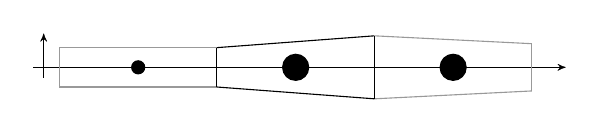
\begin{tikzpicture}[outer sep = 0pt]

%%%%%%%%%%%%%%%%%%%%%%%%%%%%%%%%%

% axis
\draw [pil,very thin] (-3.4,0) -- ( 3.5, 0);
\draw [pil,very thin] (-3.2,-0.2) -- (-3.2, 0.5);

% left volume
\draw [white!60!black] (-3,-0.25) -- (-3, 0.25);
\draw [white!60!black] (-3,-0.25) -- (-1,-0.25);
\draw [white!60!black] (-3, 0.25) -- (-1, 0.25);

% central volume
\draw (-1,-0.25) -- (-1, 0.25);
\draw (-1, 0.25) -- ( 1, 0.4);
\draw (-1,-0.25) -- ( 1,-0.4);
\draw ( 1,-0.4)  -- ( 1, 0.4);

% right volume
\draw [white!60!black] ( 1,-0.4) -- ( 3,-0.3);
\draw [white!60!black] ( 1, 0.4) -- ( 3, 0.3);
\draw [white!60!black] ( 3,-0.3) -- ( 3, 0.3);

% centroids
\path (-2, 0) node [shape=circle, draw, fill=black, scale=0.5] {}
      ( 0, 0) node [shape=circle, draw, fill=black] {}
      ( 2, 0) node [shape=circle, draw, fill=black] {};

\draw ( 1,-0.4)  -- ( 1, 0.4);

\end{tikzpicture}
\end{document}

